\sloppy
\documentclass[14pt,a4paper,oneside]{extarticle}	% Размер основного шрифта и формата листа
\usepackage{xltxtra}						% Используется для вывода логотипа XeLaTeX
\usepackage{xunicode}						% Кодировка документа
\usepackage{polyglossia}					% Загружает пакет многоязыковой верстки
\newfontfamily\russianfont{Book Antiqua}
%\setmainfont{Liberation Serif}						% Основной шрифт текста
\setmainfont{Book Antiqua}
\setdefaultlanguage{russian}				% Основной язык текста
\setotherlanguage{english}					% Дополнительный язык текста
\linespread{1}							% Межстрочный интервал выбран полуторным
\usepackage[left=2.5cm,
right=1.5cm,vmargin=2.5cm]{geometry} % Отступы по краям листа
\bibliographystyle{ugost2008}

\usepackage{xcolor}
\usepackage{hyperref}
% Цвета для гиперссылок
\definecolor{linkcolor}{HTML}{359B08} % цвет ссылок
\definecolor{urlcolor}{HTML}{799B03} % цвет гиперссылок
\hypersetup{pdfstartview=FitH,  linkcolor=linkcolor,urlcolor=urlcolor, colorlinks=true}

%---------------------------%
%---- Пакеты расширений ----%
%---------------------------%
\usepackage{xcolor}
\usepackage{hyperref}
% Цвета для гиперссылок
\definecolor{linkcolor}{HTML}{359B08} % цвет ссылок
\definecolor{urlcolor}{HTML}{799B03} % цвет гиперссылок
\hypersetup{pdfstartview=FitH,  linkcolor=linkcolor,urlcolor=urlcolor, colorlinks=true}


\usepackage{verbatim,indentfirst}
\usepackage{cite,enumerate,float}
\usepackage{amsmath,amssymb,amsthm,amsfonts}

%---------------------------%
%--- Вставка иллюстраций ---%
%---------------------------%
\usepackage{graphicx}
\usepackage{subfigure}
%\graphicspath{{Images/}}
\usepackage{fontspec}

\begin{document}
%	\pagestyle{empty} %  выключаенм нумерацию
	
	%\setcounter{page}{3}% Нумерация начинается с третьей страницы
	%\renewcommand{\contentsname}{\center{Содержание}}
	%\tableofcontents
	

	\begin{center}
		%\addcontentsline{toc}{section}{Потенциальный барьер}
		\subsection*{Скатывание двух цилиндров}
	\end{center}
		

\begin{figure}[H] 	
	\centering 	
	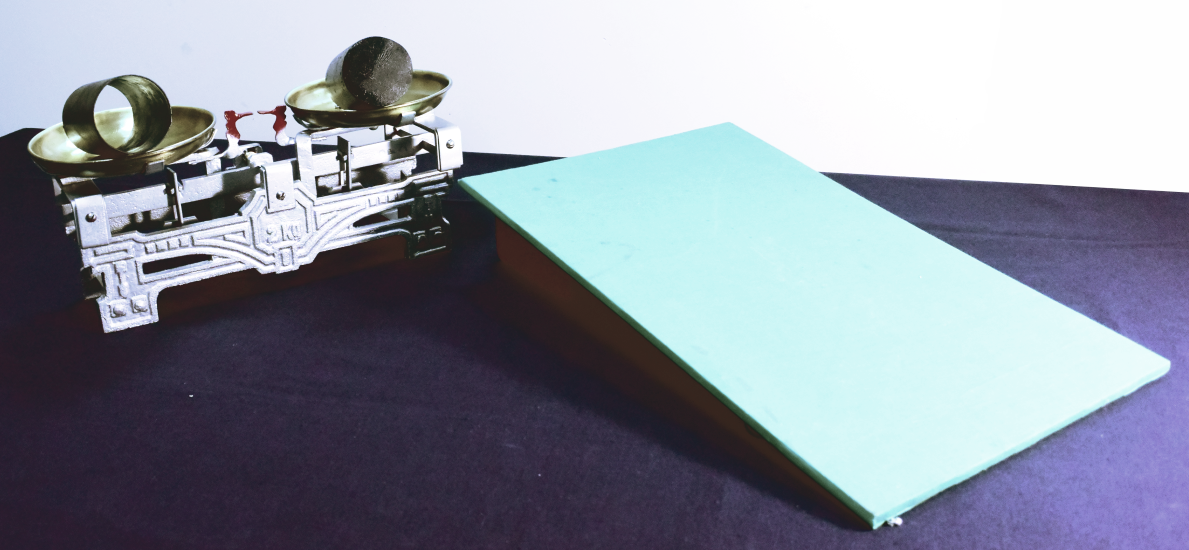
\includegraphics[width=0.9\linewidth]{inclinedplane-1.png}
	\caption{Демонстрация зависимости инертных свойств тел от распределения массы в этих телах на примере скатывания сплошного и полого цилиндров равной массы и одинакового размера с наклонной плоскости}
	\label{inclinedplane-1}
\end{figure}
	
	\subsection*{\underline{Оборудование:}}

		\begin{enumerate}
			\item Два цилиндра одинаковой массы на весах
			\item Наклонная плоскость
			\item Линейка или указка
		\end{enumerate}
		
	\subsection*{\underline{Краткое описание:}}
		
	На наклонную плоскость кладут два цилиндра одинаковой массы и радиуса.
	Цилиндры располагают так, чтобы их оси были находились одна на продолжении другой.
	
	Пустив цилиндры скатываться одновременно с наклонной плоскости, наблюдают более 
	быстрое скатывание цилиндра, масса которого сосредоточена ближе к центру, так как его момент инерции оказывается меньше.
	При этом полый цилиндр, в котором вся масса находится на значительном расстоянии от оси вращения, обладает большим моментом инерции.
	
			\begin{figure}[H] 	
		\centering 	
		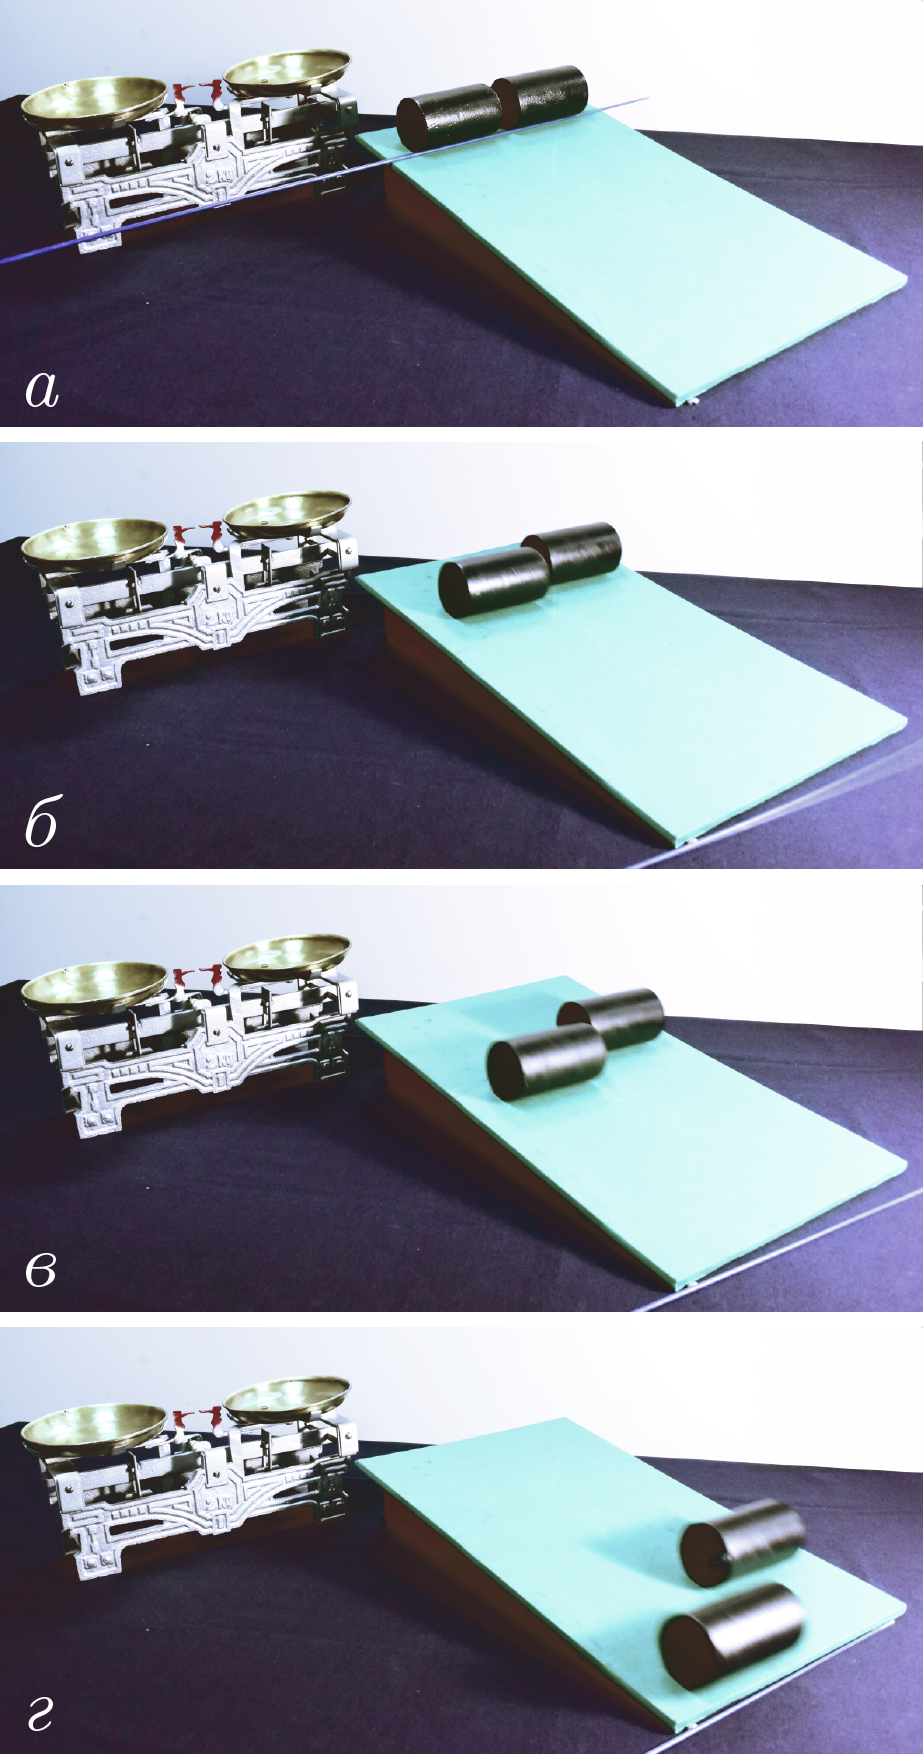
\includegraphics[width=0.5\linewidth]{inclinedplane-2.png}
		\caption{При одновременном отпускании цилиндров быстрее будет скатываться тот, чей момент инерции окажется меньше. При одинаковых размерах и массе моменты инерции двух цилиндров (сплошной и полый) будут отличаться вдвое. Из-за того, что момент инерции сплошного цилиндра в среднем оказывается меньше момента инерции полого цилиндра, с наклонной поверхности первым скатится сплошной цилиндр}
		\label{inclinedplane-2}
	\end{figure}

	Из-за разницы в распределении массы внутри скатывающихся цилиндров, их центры масс движутся вдоль наклонной плоскости с разными ускорениями.
	Опыт позволяет наглядно продемонстрировать, что чем больше момент инерции, тем медленнее изменяется линейная скорость тел при одинаковом размере и равной массе.
	
	\newpage	
	\subsection*{\underline{Теория:}}
	
	При описании движения цилиндрического тела с наклонной плоскости удобно использовать уравнение движения или второй закон Ньютона, а также записать основой закон динамики вращательного движения.
	
	\begin{figure}[H] 	
		\centering 	
		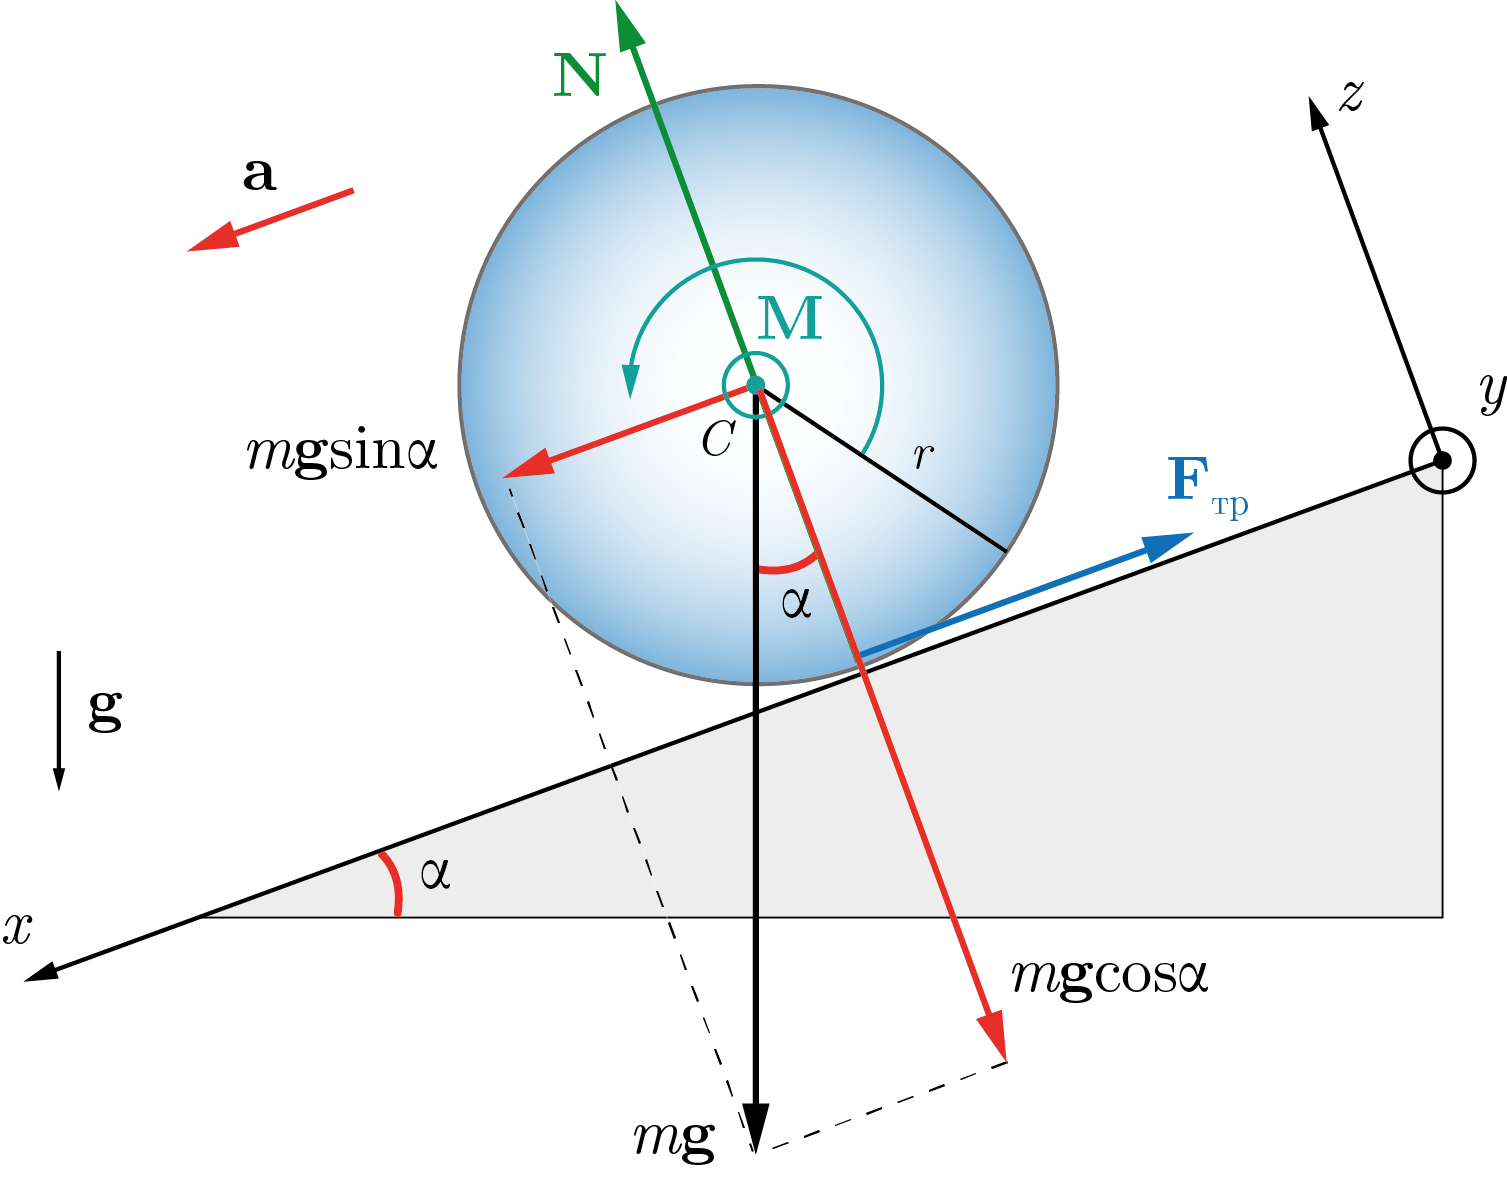
\includegraphics[width=0.8\linewidth]{inclinedplane-3.png}
		\caption{Схематичное изображение сил, действующих на цилиндр при его движении с наклонной плоскости. Сила трения создает вращательный момент, поэтому скатывающийся ускоренно цилиндр начинает закручиваться. Согласно основному закону динамики вращательного движения угловое ускорение точек цилиндра, а следовательно, и линейное ускорение его центра масс, оказывается тем больше, чем меньше его момент инерции}
		\label{inclinedplane-3}
	\end{figure}

	В векторной форме уравнение поступательного движения центра масс цилиндра запишется следующим образом:
	\begin{equation}\label{inclinedplane-1eq1}
	m\textbf{g}+\textbf{N}+\textbf{F}_{\text{тр}} = m\textbf{a}.
	\end{equation} 
	
В выбранной системе координат после проектирования всех векторов можно записать уравнение движения в скалярном виде.
В проекции на ось  \textit{x}  это уравнение примет вид:
	\begin{equation}\label{inclinedplane-1eq2}
	mg\sin\alpha - F_{\text{тр}} = ma,
	\end{equation}
	в проекции на ось  \textit{z}:
	\begin{equation}\label{inclinedplane-1eq3}
	N - mg\cos\alpha = 0.
	\end{equation}
	
	Составим основное уравнение вращательного движения относительно оси, проходящей через центр масс цилиндра. 
	Моменты силы тяжести  $	m\textbf{g} $ и реакции опоры $ \textbf{N} $ относительно этой оси равны нулю. 
	Угловое ускорение $ \textbf{ε} $ определяется только моментом силы трения $ F_{\text{тр}} $ и моментом инерции $ I $:
	\begin{equation}\label{inclinedplane-1eq4}
	 I\textbf{ε}=\textbf{M}
	\end{equation}
	где \textit{I} — момент инерции цилиндра относительно оси вращения, \linebreak $ \textbf{M} = \textbf{F}_{\text{тр}}\times \textbf{r} $ — момент силы трения, определяемый через векторное произведение силы трения на плечо.
	
	В проекции на $ y $ уравнение вращательного  движения (\ref{inclinedplane-1eq4}) примет вид:
	\begin{equation}\label{inclinedplane-1eq5}
	I\varepsilon = F_{\text{тр}} r.
	\end{equation}
	 
	Пользуясь известным соотношением между линейным и угловым ускорениями $ a = r\varepsilon $, выразим силу трения:
	\begin{equation}\label{inclinedplane-1eq6}
	F_{\text{тр}} = \frac{Ia}{r^{2}}.
	\end{equation}

	Подставляя найденную силу трения в уравнение движения (\ref{inclinedplane-1eq2}), получим:
		\begin{equation}\label{inclinedplane-1eq7}
		mg\sin\alpha -  \frac{Ia}{r^{2}} = ma.
	\end{equation}
	
	Отсюда можно выразить линейное ускорение \textit{a} центра масс скатывающегося цилиндра  

	\begin{equation}\label{8}
	a=  \frac{mg\sin\alpha}{I\textfractionsolidus r^{2} + m}  = \frac{g\sin\alpha}{1 + I/mr^{2}}.
	\end{equation} 
	  
	  Из полученного выражения следует, что изменение скорости твердого тела при движении по наклонной плоскости зависит от его момента инерции.
	 Увеличение момента инерции твердого тела приводит к уменьшению ускорения центра масс тела.
	 Таким образом, сплошной цилиндр, обладающий меньшим моментом инерции (вся его масса распределена вблизи оси вращения и момент инерции равен $ I_{1} = mr^{2}/2 $), скатывается быстрее, по сравнению с тонкостенным полым цилиндром, у которого масса в основном находится на периферии ($ I_{2} = mr^{2}  $).    
	
\end{document}
